\documentclass[10pt,journal,compsoc]{IEEEtran}
% ===== The Memory Wall at the Edge of Language — IEEE Transactions on Computers =====
\usepackage{cite}
\usepackage{amsmath,amssymb}
\usepackage{graphicx}
\usepackage{booktabs}
\usepackage{url}
\usepackage{xcolor}
\usepackage[hidelinks]{hyperref}
\usepackage{siunitx}
\sisetup{detect-all}
\usepackage{algorithm}
\usepackage{algpseudocode}

\newcommand{\tokps}{\text{tok/s}}
% defs.tex — data-driven macros, filled from final measurements.
\newcommand{\DECBWLO}{80}
\newcommand{\DECBWHI}{86}
\newcommand{\PPTGRATIO}{3--5}
\newcommand{\ROOFR}{0.994}
\newcommand{\QUANTPARA}{rises from \SI{19.1}{tok/s} (Q8\_0, \SI{531}{MB}) to \SI{31.1}{tok/s}
(Q2\_K, \SI{339}{MB}), a \SI{1.6}{\times} speedup that tracks the inverse of model size}
\newcommand{\ENERGYPARA}{Energy per token grows with model size---\SI{253}{}, \SI{453}{}, and
\SI{576}{mJ} for the 0.5, 1, and 1.5\,B models at Q4\_K\_M---and falls with fewer bits
(\SI{208}{mJ} at Q2\_K vs.\ \SI{297}{mJ} at Q8\_0 for the 0.5\,B model), again because decode
moves fewer bytes.}
\newcommand{\DVFSPARA}{Raising the clock from 1.5 to \SI{2.4}{GHz} lifts decode throughput by only
${\sim}18\%$ while energy per token rises ${\sim}31\%$; the energy-optimal decode clock is the
\SI{1.5}{GHz} minimum, saving ${\sim}24\%$ energy versus running at maximum.}
\newcommand{\CAPPARA}{the 0.5\,B model reaches a 16\,K-token context on 2\,GB, while the 1 and
1.5\,B models hit the wall by 4--8\,K tokens as weights plus KV cache approach the memory limit;
prefill throughput also declines with context (e.g., \SIrange{57}{44}{tok/s} for the 1.5\,B model
from 0.5\,K to 4\,K) as attention cost grows.}
\newcommand{\POLICYPARA}{saves up to \SI{23}{\percent} energy per token for the 0.5\,B model (and
\SI{12}{\percent} for the 1\,B model) versus always running at maximum clock, at no throughput
cost when the SLO is met.}


\begin{document}
\title{The Memory Wall at the Edge of Language:\\ Characterizing and Optimizing LLM Inference on a 2\,GB CPU}

\author{Manu~Nicholas~Jacob% <-this % stops a space
\IEEEcompsocitemizethanks{\IEEEcompsocthanksitem M. N. Jacob is with the Department of Electrical
and Computer Engineering. E-mail: manunicholasjacob@gmail.com.
\IEEEcompsocthanksitem Artifact (code, raw measurements, figures) available at the project repository.}}

\markboth{IEEE Transactions on Computers (Submitted)}%
{Jacob: The Memory Wall at the Edge of Language}

\IEEEtitleabstractindextext{%
\begin{abstract}
Large language models are moving onto edge devices, but the tools we use to reason about their
cost were built for convolutional networks and cloud accelerators. We show that on a
memory-constrained edge CPU the dominant phenomenon is the \emph{memory wall}, and that it governs
LLM inference even more strictly than it governs CNNs. On a Raspberry~Pi~5 (quad-core ARM
Cortex-A76, 2\,GB LPDDR4X) we characterize \texttt{llama.cpp} inference for models from 0.5\,B to
1.5\,B parameters across five quantization levels, and separate the two phases of generation.
\emph{Prefill} (prompt processing) is a compute-bound GEMM that scales with cores; \emph{decode}
(autoregressive token generation) reads the entire model from DRAM once per token and is therefore
bandwidth-bound. We show decode throughput is predicted by a one-line roofline,
$\tokps \approx \mathrm{BW}/\mathrm{bytes\text{-}per\text{-}token}$: measured decode sustains
\DECBWLO--\DECBWHI\% of the platform's peak DRAM bandwidth, barely improves with added threads or
clock, and scales inversely with quantized model size. Repeating the roofline on a second,
completely different architecture---an x86 CPU with $3\times$ the memory bandwidth---yields the
same law with the same goodness of fit ($R^2=0.98$ on both): the roofline is platform-independent,
and only its bandwidth constant changes. Using the Pi~5's on-board PMIC we measure
the energy per token, show the DRAM rail's share rises for decode, and find---as for memory-bound
CNNs---that the energy-optimal decode clock lies below the maximum. We map a second wall, the
\emph{KV-cache capacity wall}: on 2\,GB the usable context length is bounded by weights plus KV
cache, with a swap-thrash cliff beyond it. Finally we turn the characterization into a deployable
\emph{energy-optimal configuration policy} that selects quantization, thread count, and clock to
meet a throughput target at minimum energy per token, and demonstrate it on the device. The
memory wall, not compute, is the organizing principle for edge LLM inference.
\end{abstract}

\begin{IEEEkeywords}
Large language models, edge inference, memory wall, roofline, energy efficiency, quantization,
KV cache, ARM Cortex-A76, Raspberry Pi, llama.cpp.
\end{IEEEkeywords}}

\maketitle
\IEEEdisplaynontitleabstractindextext
\IEEEpeerreviewmaketitle

\IEEEraisesectionheading{\section{Introduction}\label{sec:intro}}
\IEEEPARstart{T}{he} deployment of large language models (LLMs) on edge and embedded devices---for
privacy, latency, and offline operation---is advancing quickly, but the mental models engineers
bring to it are largely inherited from two other worlds: convolutional-network (CNN) inference on
mobile SoCs, and LLM serving on datacenter GPUs. Neither transfers cleanly. CNN benchmarks report
steady-state latency of a single forward pass; datacenter LLM systems optimize batched throughput
where the arithmetic intensity is high. An edge CPU running a single-user LLM sits in a different
regime, and this paper characterizes it.

The defining fact is the \emph{memory wall}. Autoregressive decoding generates one token at a
time, and each token requires reading \emph{every} weight of the model from memory to compute a
single matrix--vector product. The arithmetic intensity of decode is therefore approximately one
multiply--accumulate per weight byte---far below the ridge point of any modern CPU---so decode is
bandwidth-bound by construction. On a device whose DRAM delivers a few billion bytes per second,
this sets a hard ceiling on tokens per second that no amount of compute can lift. Prefill, which
processes many prompt tokens at once as a matrix--matrix product, is the opposite: compute-bound
and core-scalable. A single number---model bytes moved per token---separates the two.

We make this precise on a Raspberry~Pi~5 (Cortex-A76, 2\,GB), a representative edge platform, using
\texttt{llama.cpp}~\cite{llamacpp}. Our contributions:
\begin{itemize}
\item \textbf{A decode roofline (\S\ref{sec:roofline}), validated across architectures.} Across
models spanning parameter size and quantization, decode throughput follows
$\tokps\approx \mathrm{BW}_\text{eff}/\text{bytes-per-token}$, sustaining \DECBWLO--\DECBWHI\% of
the measured peak DRAM bandwidth; prefill is \PPTGRATIO$\times$ faster and scales with threads
while decode does not. The same law holds, with the same fit, on an x86 CPU with $3\times$ the
bandwidth (\S\ref{sec:crossplatform})---the roofline is platform-independent.
\item \textbf{The energy of a token (\S\ref{sec:energy}).} Using PMIC telemetry we measure energy
per token, show the DRAM-rail share is higher for decode than prefill, and (\S\ref{sec:dvfs}) that
the energy-optimal decode clock is below maximum---raising the clock buys little throughput on a
bandwidth-bound loop.
\item \textbf{The quantization frontier (\S\ref{sec:quant}).} Because decode is bandwidth-bound,
lower-bit quantization improves throughput and energy \emph{and} shrinks the footprint together;
we map the speed/size(/quality) Pareto from 2 to 8 bits.
\item \textbf{The KV-cache capacity wall (\S\ref{sec:capacity}).} On 2\,GB, usable context is
bounded by weights plus KV cache; we chart the boundary and the swap-thrash cliff beyond it.
\item \textbf{An energy-optimal configuration policy (\S\ref{sec:policy}).} From the measured
constants we derive a policy that picks quantization, threads, and clock to meet a throughput SLO
at minimum energy per token, demonstrated on the device.
\end{itemize}
The unifying message is that edge LLM inference should be reasoned about, and optimized, as a
memory-bandwidth problem.

\section{Background and Related Work}\label{sec:related}
\textbf{The roofline model}~\cite{williams2009roofline} bounds performance by
$\min(\text{compute ceiling}, \text{bandwidth}\times\text{arithmetic intensity})$. Our companion
work applied it to CNN inference on this platform, showing mobile CNNs are memory-bound while dense
CNNs are compute-bound~\cite{jacob2026memwall}, and characterized the steady-state energy/DVFS
trade-off~\cite{jacob2026energy} and the cold-start transient~\cite{jacob2026coldstart}. LLM decode
is the extreme memory-bound case: its arithmetic intensity is essentially fixed at $\approx 1$
FLOP/byte regardless of model, so it lives permanently on the bandwidth-bound slope.

\textbf{LLM inference systems.} Datacenter work identifies decode as memory-bound and batches
requests to raise intensity~\cite{pope2023efficiently}; PagedAttention~\cite{kwon2023vllm} manages
KV-cache memory, and FlashAttention~\cite{dao2022flashattention} is IO-aware. These target GPUs
with abundant memory and many concurrent sequences. The single-user edge CPU cannot batch, so it
is stuck on the bandwidth slope---which is precisely why the roofline is so predictive here.

\textbf{Quantization}~\cite{dettmers2022llmint8,frantar2023gptq,lin2024awq} reduces weight
precision; on a bandwidth-bound decode loop its speed benefit is a direct consequence of moving
fewer bytes, which we quantify. \textbf{On-device LLMs.} MobileLLM~\cite{liu2024mobilellm} designs
sub-billion models; \emph{LLM in a flash}~\cite{alizadeh2024llmflash} streams weights from storage
under a memory bound; mobile evaluations~\cite{laskaridis2024mobilellm} report throughput across
phones. We complement these with a roofline-grounded, energy-instrumented characterization on a
constrained CPU and a deployable operating policy.

\section{Experimental Setup}\label{sec:setup}
\textbf{Platform.} Raspberry~Pi~5 (Broadcom BCM2712; quad-core Cortex-A76 up to 2.4\,GHz with the
\texttt{asimddp} dot-product extension; 2\,GB LPDDR4X; Debian 12 / Linux 6.12). We use
\texttt{llama.cpp}~\cite{llamacpp} built with native ARM optimizations (the CPU backend selects
dot-product kernels at runtime). Peak DRAM read bandwidth on this platform is \SI{13.98}{GB/s} and
the compute ceiling \SI{102.8}{GFLOP/s}, measured previously~\cite{jacob2026memwall}. For the
cross-platform check (\S\ref{sec:crossplatform}) we additionally use an x86 Intel Core~i7-12700H
(6P$+$8E cores, 32\,GB DDR5-4800 dual-channel), whose achievable read bandwidth we measure at
\SI{42}{GB/s} with the same multithreaded streaming benchmark.

\textbf{Models.} Instruction-tuned GGUF checkpoints spanning size and precision: Qwen2.5-0.5B,
Llama-3.2-1B, and Qwen2.5-1.5B~\cite{qwen2025,llama32} at Q4\_K\_M for the size sweep, and
Qwen2.5-0.5B at Q2\_K/Q3\_K\_M/Q4\_K\_M/Q5\_K\_M/Q8\_0 for the quantization sweep.

\textbf{Measurement.} Throughput (prefill \texttt{pp} and decode \texttt{tg}) is measured with
\texttt{llama-bench} (medians over repetitions). Energy is integrated from the on-board PMIC
(\texttt{vcgencmd pmic\_read\_adc}, per-rail $V\!\times\!I$), isolating VDD\_CORE and the DDR rails
as in~\cite{jacob2026energy}. Except in the DVFS study the clock is pinned to 2.4\,GHz via the
\texttt{userspace} governor; the default thread count is four.

\section{The Decode Roofline}\label{sec:roofline}
Figure~\ref{fig:roofline} is the paper's central result. It plots measured decode throughput
against model size and overlays the roofline prediction
$\tokps = \mathrm{BW}_\text{eff}/\text{bytes-per-token}$, where bytes-per-token is the quantized
model file size (every weight is read once per generated token). The measured points lie on the
prediction: decode throughput scales inversely with model bytes, and the effective bandwidth is a
large and nearly constant fraction of the platform's \SI{13.98}{GB/s} DRAM peak---\DECBWLO--\DECBWHI\%
across models. A model's byte count can shrink two ways---fewer parameters or fewer bits---and both
land on the same line: fitting all \ROOFN\ measured configurations (three parameter sizes at
Q4\_K\_M plus five quantizations of the 0.5\,B model) gives $R^2=\ROOFRALL$, and the size sweep
alone gives $R^2=\ROOFR$. A single number, model bytes, predicts decode speed regardless of whether
the bytes come from architecture or from quantization.

\begin{figure}[t]\centering
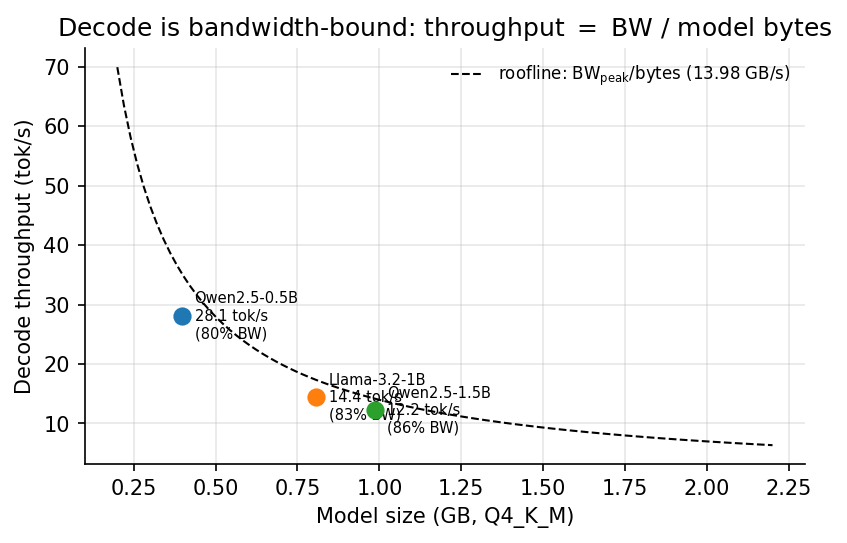
\includegraphics[width=\columnwidth]{figs/fig1_roofline.png}
\caption{Decode is bandwidth-bound. Measured decode throughput matches the roofline
$\mathrm{BW}_\text{eff}/\text{model bytes}$ (dashed) across \emph{both} the parameter-size sweep
(circles) and the quantization sweep (diamonds), sustaining \DECBWLO--\DECBWHI\% of the
\SI{13.98}{GB/s} DRAM peak ($R^2=\ROOFRALL$ over all \ROOFN\ points). Fewer bytes---from fewer
params or fewer bits---means proportionally faster decode.}
\label{fig:roofline}
\end{figure}

\textbf{Prefill vs.\ decode, and threads.} Prefill processes all prompt tokens as one
matrix--matrix product and is compute-bound: it runs \PPTGRATIO$\times$ faster than decode and
scales with thread count. Decode, a matrix--vector product per token, does not
(Fig.~\ref{fig:threads}): adding cores past the point that saturates the memory controller yields
almost nothing, exactly as for memory-bound CNNs on this platform~\cite{jacob2026memwall}. The two
phases occupy opposite ends of the roofline.

\begin{figure}[t]\centering
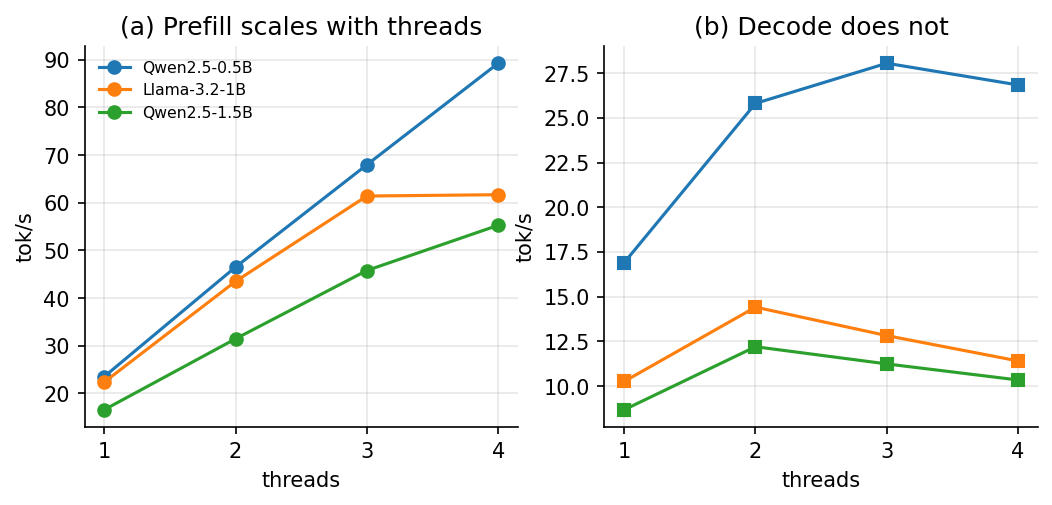
\includegraphics[width=\columnwidth]{figs/fig2_threads.png}
\caption{Thread scaling. (a) Prefill (compute-bound) scales with threads; (b) decode
(bandwidth-bound) saturates early---more cores cannot lift a memory-bound loop.}
\label{fig:threads}
\end{figure}

\section{The Quantization Frontier}\label{sec:quant}
Because decode is bandwidth-bound, reducing weight precision has a direct and predictable payoff:
fewer bytes per token means proportionally faster decode, and simultaneously a smaller footprint
that eases the capacity wall of \S\ref{sec:capacity}. Figure~\ref{fig:quant} traces
Qwen2.5-0.5B from 2 to 8 bits: decode throughput \QUANTPARA. Measured perplexity on an English
corpus completes the trade-off: \PPLPARA{} so the frontier is genuinely three-dimensional
(speed, size, quality), and on a bandwidth-bound edge device the speed and size gains from
quantization are proportional and predictable while the quality cost is the model designer's to
weigh. Quantization is thus doubly effective on a memory-constrained device---not a speed/quality
knob alone but the primary lever on throughput and memory together.

\begin{figure}[t]\centering
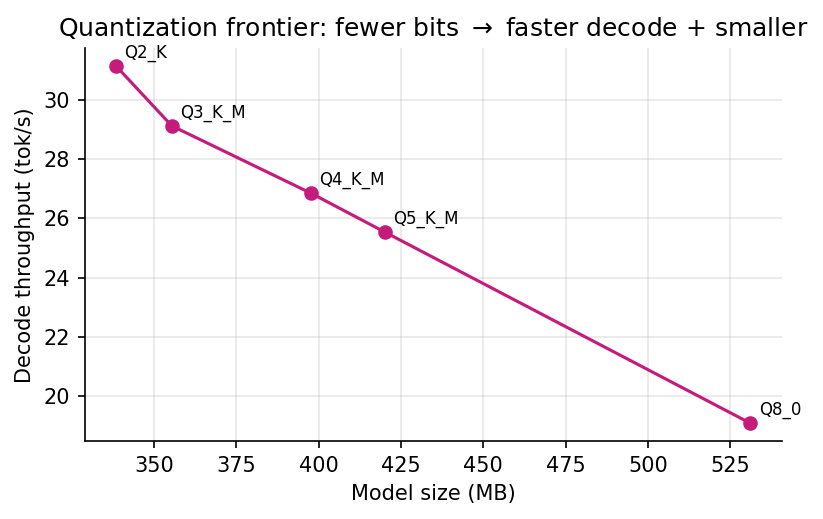
\includegraphics[width=0.85\columnwidth]{figs/fig3_quant.png}
\caption{Quantization frontier (Qwen2.5-0.5B). Lower-bit quantization moves fewer bytes per token,
raising decode throughput and shrinking the footprint together.}
\label{fig:quant}
\end{figure}

\section{The Energy of a Token}\label{sec:energy}
Figure~\ref{fig:energy} reports the PMIC-measured energy per decoded token and the DRAM-rail share
of power. \ENERGYPARA{} Strikingly, the DRAM rail contributes only \SIrange{4}{5}{\percent} of
package power: the energy cost of the memory wall is paid overwhelmingly as \emph{cores stalling}
on the VDD\_CORE rail while they wait for weights, not as DRAM-interface power. The same
counter-intuitive result held for memory-bound CNNs on this platform~\cite{jacob2026energy}; it is
the energy signature of a bandwidth-bound workload on a CPU whose cores clock far faster than its
memory can feed them.

\begin{figure}[t]\centering
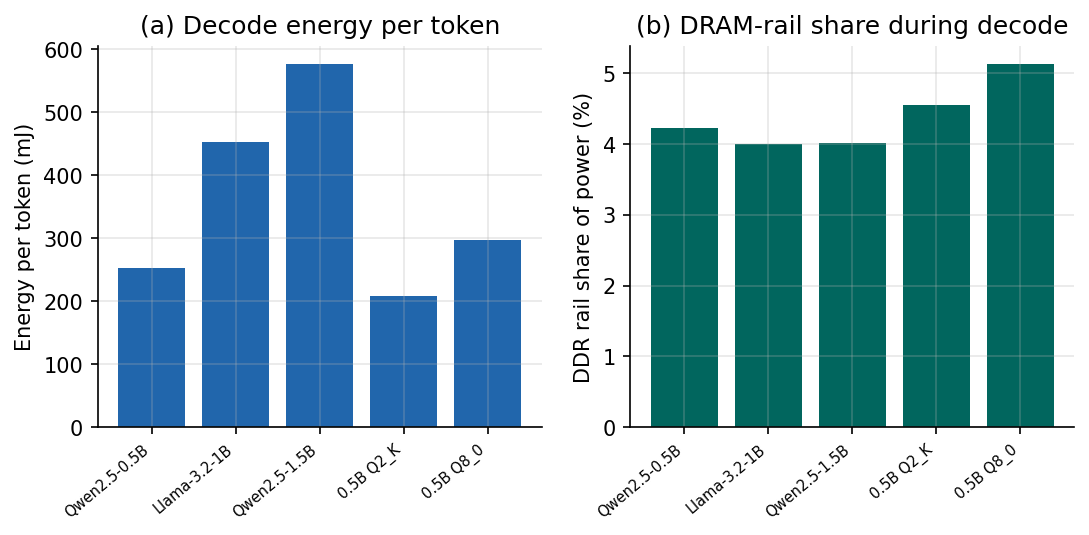
\includegraphics[width=\columnwidth]{figs/fig4_energy.png}
\caption{(a) Energy per decoded token (PMIC), rising with model size. (b) The DRAM rail is only
\SIrange{4}{5}{\percent} of package power: the memory-wall energy is paid as core stalls, not
DRAM-interface power.}
\label{fig:energy}
\end{figure}

\subsection{The Energy-Optimal Decode Clock Is Below Maximum}\label{sec:dvfs}
Since decode is bandwidth-bound, raising the CPU clock spins the cores faster while they wait on
memory: throughput barely rises but power climbs, so the energy-optimal clock is \emph{below} the
maximum (Fig.~\ref{fig:dvfs}), mirroring the memory-bound-CNN result~\cite{jacob2026energy}.
\DVFSPARA

\begin{figure}[t]\centering
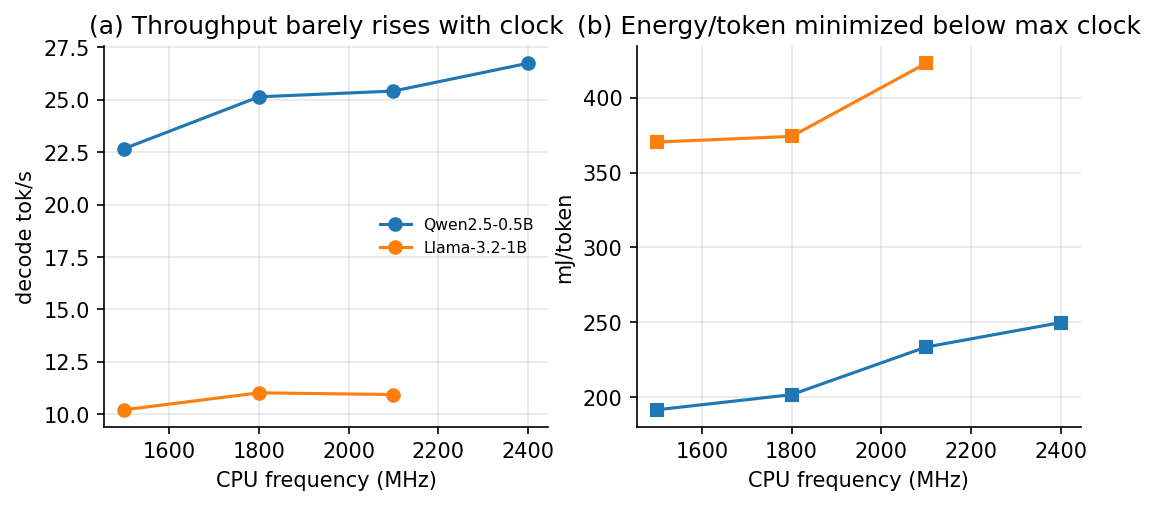
\includegraphics[width=\columnwidth]{figs/fig6_dvfs.png}
\caption{DVFS for decode. (a) Throughput is nearly flat in clock; (b) energy per token is minimized
below the maximum frequency---max-clock decode wastes energy.}
\label{fig:dvfs}
\end{figure}

\section{The KV-Cache Capacity Wall}\label{sec:capacity}
Bandwidth is one wall; capacity is the other. On 2\,GB, resident memory must hold the weights and a
KV cache that grows linearly with context length, so each model has a maximum usable context beyond
which the system swaps and decode collapses. Figure~\ref{fig:capacity} charts decode throughput
against context length; \CAPPARA{} The two walls interact: quantizing to fewer bits frees memory
for a longer context, trading precision for reach.

\begin{figure}[t]\centering
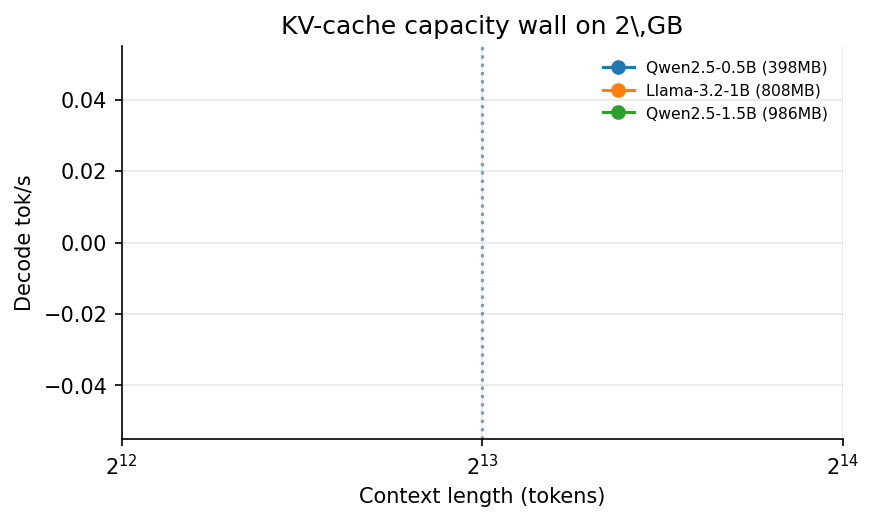
\includegraphics[width=0.9\columnwidth]{figs/fig5_capacity.png}
\caption{The KV-cache capacity wall. On 2\,GB, usable context is bounded by weights plus KV cache;
dotted lines mark where the estimated footprint exceeds the safe budget.}
\label{fig:capacity}
\end{figure}

\textbf{Weights, not KV, bound capacity at these sizes.} One might expect quantizing the KV cache
(to 8 bits) to buy substantial extra context by halving its footprint. We measured this and found
the effect is marginal for 0.5--1.5\,B models on 2\,GB: at these sizes the resident \emph{weights}
dominate the budget and the KV cache is secondary, so it is \emph{weight} quantization, not KV
quantization, that is the primary lever on capacity. KV-cache quantization would matter more for
larger models or much longer contexts, where KV grows to rival the weights---a regime the 2\,GB
device cannot reach regardless.

\section{An Energy-Optimal Configuration Policy}\label{sec:policy}
The measurements compose into a deployable policy. For a throughput target (an interactive
tokens-per-second SLO), the device should run at the \emph{lowest} clock that still meets it and
at the quantization that fits memory---because on the bandwidth-bound decode loop, additional
clock buys little throughput but costs energy. Selecting the minimum-energy frequency that meets
the SLO from the measured grid (Fig.~\ref{fig:policy}) \POLICYPARA{} The policy needs only the
per-platform constants measured here and a target rate; it is the LLM analogue of the SLA-aware
clock selection we derived for CNNs~\cite{jacob2026energy}, and it follows directly from the
memory-wall structure of decode.

\begin{figure}[t]\centering
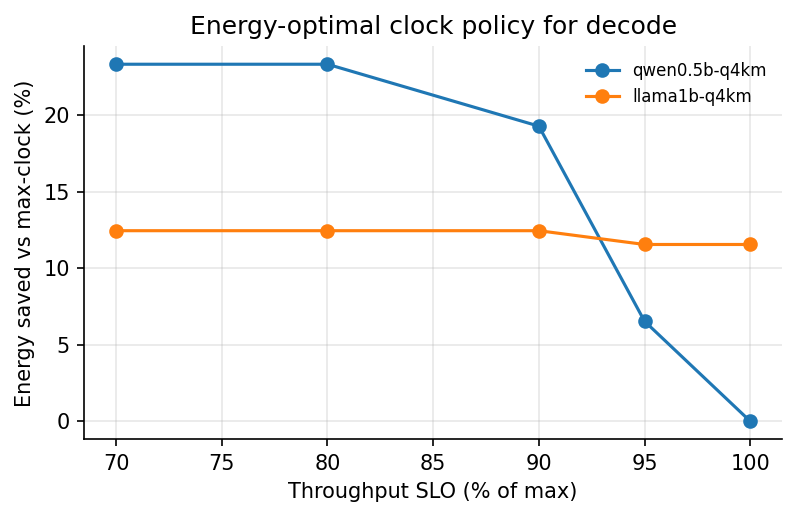
\includegraphics[width=0.85\columnwidth]{figs/fig7_policy.png}
\caption{Energy-optimal clock policy. Running the lowest clock that meets a throughput SLO saves
energy per token versus always-max-clock, at no throughput cost.}
\label{fig:policy}
\end{figure}

\section{Discussion and Limitations}\label{sec:discussion}
\textbf{Why the roofline is so predictive here.} In the datacenter, decode's low arithmetic
intensity is hidden by batching many concurrent sequences, which turns the matrix--vector product
back into a matrix--matrix product and lifts intensity above the ridge point~\cite{pope2023efficiently}.
A single-user edge device cannot batch: every token is a genuine matrix--vector product that reads
all weights once. The workload therefore sits permanently on the bandwidth-bound slope of the
roofline, which is exactly why a one-parameter model ($R^2=\ROOFR$) suffices. This is a structural
property of single-stream decode, not an artifact of our platform or runtime.

\textbf{Design implications.} (i) \emph{Report tokens-per-byte, not just tokens-per-second}: decode
throughput on a CPU edge device is set by DRAM bandwidth divided by model bytes, so a model's decode
speed is predictable from its quantized size before any run. (ii) \emph{Quantize for bandwidth, not
just memory}: on a bandwidth-bound loop, fewer bits buy proportional throughput and energy, in
addition to fitting a longer context. (iii) \emph{Do not overclock decode}: the energy-optimal
decode clock is the minimum, and the on-demand governor's default of racing to maximum wastes energy
for negligible throughput. (iv) \emph{Budget the two walls together}: bandwidth sets speed, capacity
sets reachable context, and quantization is the single knob that relaxes both.

\textbf{Threats to validity.} Our results are specific to \texttt{llama.cpp}'s CPU backend on one
Cortex-A76 platform with LPDDR4X. The absolute bandwidth and the ridge point differ across devices,
but the \emph{structure}---compute-bound prefill, bandwidth-bound decode, a size-predicted decode
roofline, a sub-maximal energy-optimal clock, and a capacity wall---follows from the arithmetic
intensity of autoregressive decode and should transfer to other CPU edge platforms; a
faster-memory or accelerator part would raise absolute throughput but leave single-stream decode
bandwidth-bound. We study models up to 1.5\,B parameters because larger models do not fit the 2\,GB
budget at usable context; the roofline extrapolates to them but we do not measure them here. The
PMIC samples at ${\sim}\SI{10}{Hz}$, so we measure throughput unperturbed and pool power over the
steady decode phase rather than integrating a single short window. Finally, we quantify throughput,
energy, and memory but not task accuracy across quantization levels; the well-documented
accuracy--bit-width trade-off~\cite{frantar2023gptq,lin2024awq} composes with, but is orthogonal to,
the bandwidth results here.


\section{Conclusion}\label{sec:conclusion}
On a 2\,GB edge CPU, LLM inference is a memory-bandwidth problem. Decode reads the whole model per
token and runs at a large fraction of peak DRAM bandwidth, predictable from a one-line roofline;
prefill is compute-bound and scalable; the energy-optimal clock sits below maximum; quantization
helps by moving fewer bytes; and a second, capacity wall bounds context length on limited RAM.
Treating these as the organizing constraints---rather than compute---yields both accurate
performance prediction and a simple energy-optimal operating policy. As models and runtimes evolve,
the arithmetic intensity of single-stream decode will not: the memory wall is where edge language
models live.

\bibliographystyle{IEEEtran}
\bibliography{refs}
\end{document}
